	\section{\textbf{LiDAR}} El LiDAR (acrónimo de Light Detection and Ranging) es una tecnología de teledetección que utiliza pulsos de luz láser para medir distancias y movimientos precisos en un entorno en tiempo real. Esta técnica permite generar mapas topográficos detallados y modelos 3D de alta precisión, siendo esencial en aplicaciones como la navegación de vehículos autónomos y la evaluación de riesgos naturales.
\subsection{\textbf{¿Cómo funciona LiDAR?}}
El sistema LiDAR funciona midiendo el tiempo que tarda un pulso de luz láser en viajar desde el sensor hasta un objeto y regresar. Dado que la velocidad de la luz es constante, este tiempo de recorrido permite calcular la distancia con gran precisión.

\subsubsection{\textbf{Componentes Principales}}
\begin{itemize}
	\item \textbf{Escáner láser}: Emite pulsos de luz infrarroja.
	\item \textbf{Sensor LiDAR}: Recoge los pulsos reflejados en los objetos del entorno.
	\item \textbf{Procesador}: Calcula la distancia basada en el tiempo de retorno del pulso y genera una nube de puntos tridimensional.
\end{itemize}

El proceso se repite millones de veces por segundo, generando un mapa tridimensional detallado del entorno. Estos datos pueden ser usados en simulaciones, sistemas de navegación y modelado del terreno.
\subsection{\textbf{¿Para qué sirve LiDAR?}}
El LiDAR tiene una amplia gama de aplicaciones en diversas industrias:

\subsubsection{\textbf{Agricultura}}
\begin{itemize}
	\item Mide la topografía de los terrenos agrícolas.
	\item Permite estimar la biomasa de los cultivos y detectar propiedades del suelo.
\end{itemize}

\subsubsection{\textbf{Aeroespacial y Defensa}}
\begin{itemize}
	\item Se usa para mapear terrenos con alta precisión.
	\item Rastrea objetivos y apoya la planificación de misiones militares.
\end{itemize}

\subsubsection{\textbf{Automoción}}
\begin{itemize}
	\item Es clave en la navegación de vehículos autónomos.
	\item Mejora la seguridad mediante la detección y análisis del entorno en tiempo real.
\end{itemize}

\subsubsection{\textbf{Silvicultura}}
\begin{itemize}
	\item Permite mapear el dosel forestal con gran detalle.
	\item Ayuda en la gestión y conservación de recursos forestales.
\end{itemize}

\subsubsection{\textbf{Geología y Minería}}
\begin{itemize}
	\item Se usa para la cartografía de minas y yacimientos.
	\item Optimiza la planificación de operaciones mineras.
\end{itemize}
\begin{figure}[H]
	\centering
	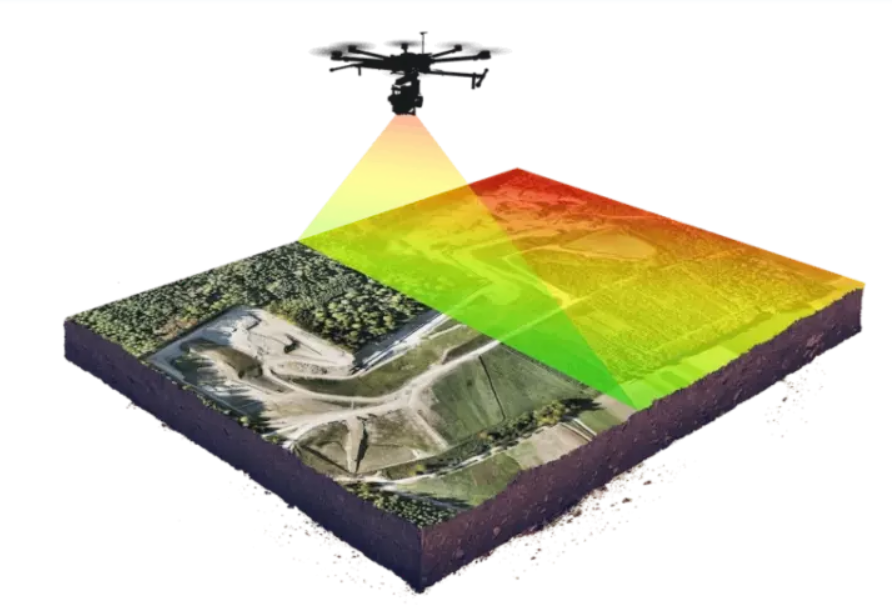
\includegraphics[width=0.35\textwidth]{lidar.png}
	\caption{LiDAR}
\end{figure}
